\documentclass[8pt,journal,compsoc]{IEEEtran}
\usepackage[pdftex]{graphicx}
\usepackage{amsfonts}
\begin{document}

\title{Alpha-Stable Distributions and Saccadic Foraging}

\author{William Edward Hahn, Elan Barenholtz% <-this % stops a space
\IEEEcompsocitemizethanks{\IEEEcompsocthanksitem W. E. Hahn is with the Center for Complex Systems and Brain Sciences at Florida Atlantic University, FL, 33431 \protect\\
E-mail: see http://www.ccs.fau.edu/$\sim$hahn/
\IEEEcompsocthanksitem Elan Barenholtz is with the Department of Psychology and the Center for Complex Systems and Brain Sciences at Florida Atlantic University, FL, 33431 \protect\\
E-mail: see http://psy2.fau.edu/~barenholtz/}% <-this % stops a space
\thanks{Manuscript received January 14, 2014; revised January 14, 2014.}}




\markboth{FAU - Spring 2014}%
{Hahn \MakeLowercase{\textit{et al.}}: Alpha-Stable Distributions}






\IEEEcompsoctitleabstractindextext{%
\begin{abstract}




\end{abstract}

\begin{IEEEkeywords}
Alpha-Stable, Levy, Foraging, HVS, Search, Visual Saliency
\end{IEEEkeywords}}


\maketitle


\IEEEdisplaynotcompsoctitleabstractindextext

\IEEEpeerreviewmaketitle

%\onecolumn

\section{Introduction}


Alpha-stable distributions are a family of four parameter heavy-tail distributions that generalize the normal distribution and have been shown to be advantageous when searching for randomly and sparsely distributed resources. Research remains limited because closed form analytic expressions for these non-Gaussian distributions are not available. Recently these curves have characterized in the frequency domain and efficient algorithms involving Fast Fourier Transform (FFT) have been developed to numerically approximate these expressions.  An optimal foraging strategy must balance intensification with diversification, exploration with exploitation, searching around the current solutions while making sure to explore the space efficiently. Research gathering animal behaviors of many species show that foragers try to minimize the distance travelled between targets to maximize their energy gain. Gaze shifts in the human visual system (HVS) can be thought of as the visual system foraging for areas rich in visual saliency. The visual system must decide when an image region has undergone sufficient processing to move to a new location. Given the limited perceptive range and informational capacity of the visual system, what is an optimal eye-movement strategy? While previous research has considered which image locations are informationally rich, much less research has considered general factors of saccadic movements, such as how often and how far the eyes should move under an optimal information-gathering strategy. Statistical models show overlap between simple animal foraging and gaze relocation. In this work, we develop new graphics processing units (GPU) techniques for the estimation of alpha-stable distribution parameters. There are many methods for fitting alpha-stable distributions and mixtures of alpha-stable distributions.The FFT provides a convent and fast method for approximating alpha-stable distributions. For Maximum Likelihood Estimation Methods (MLE) many FFT would be required thus justifying the use of the GPU. These high speed numerical methods allow of for the fitting alpha-stable parameters to a variety of HVS measurements including the focus here: saccadic distributions. Eye tracking data is typically first characterized by a thresholding into fixations and saccades and the two data subsets are then analyzed separately. Here we employ recently developed numerical techniques that allow for the characterization of distributions with heavy tails. This modern characterization allows the entire dataset to be analyzed as a whole. The primary parameter of interest is the first parameter alpha $alpha$. This parameter determines how heavy the tail of the distribution will be. For example for $\alpha=2$ we have the special case of the Gaussian curve, with this normal distribution we would not expect many samples more than 3 sigma from the mean, with a heavy tail distribution $\alpha<2$ there will be a nonzero chance of finding a sample many times the standard deviation from the mean. Intuitively this means that most samples will be close zero and everyone once in a while there is a very large sample drawn. Many natural systems behave in this manner with a many small changes punctuated infrequently by very large events.Data suggests that eye movement distributions are well described by alpha-stable distributions and thus do not have closed form solutions and should be characterized by numerical approximations of stable distributions. With a higher resolution in the fovea and limited processing resources we can think of visual saccades as a searching mechanism. Visual search is analogous to animal foraging in the sense that it is not feasible to sample the entire search space and limited resources constrain the behavior. The HVS is foraging for information rich or salient regions and because resources are limited the sensing mechanism must compress the data stream as it is sampled. Human scanpath behavior can thus be thought of as a search strategy or infotaxis mechanism. Heuristic search is a branch of soft computing in the sense that rigorous proofs are not available to guarantee that the algorithm will terminate with a solution. Often in many real world problems exact solutions are often not necessary and feasible or potentials solution are desired. For many interesting problems a potential solution can be validated in polynomial time but the generation of a optimal solution can be exponential in its running time. Even for fitness functions that will run in polynomial time it is still prohibitive to brute force the design space to find the optimal solution. For even many trivial tasks, the curse of dimensionality ensures that systematic Cartesian search will never pan out. Modern heuristic search algorithms rely on the injection of outside noise for the generation of potential solutions. Could it be that the HVS also inject noise into the search procedure? If so, what type of noise would be ideal? In the mathematical optimization algorithms alpha-stable distributions have been shown to be advantageous in n-dimensional search. This work is an attempt to characterize human saccade and scan path behavior and identify task specific and subject differences. The HVS is able to traverse larges swaths of the fitness (saliency) landscape quickly and settle on a solution. 




\section{MMS}
The Methodology, Measurement, and Statistics (MMS) Program is an interdisciplinary program in the Social, Behavioral, and Economic Sciences that supports the development of innovative analytical and statistical methods and models for those sciences. 

MMS seeks proposals that are methodologically innovative, grounded in theory, and have potential utility for multiple fields within the social and behavioral sciences.  

As part of its larger portfolio, the MMS Program partners with a consortium of federal statistical agencies to support research proposals that further the development of new and innovative approaches to surveys and to the analysis of survey data.















\cite{kennedy2010particle}
\cite{yang2009cuckoo}
\cite{yang2010firefly}
\cite{gandomi2013cuckoo}
\cite{yang2010eagle}
\cite{yang2013computational}
\cite{pomerleau1989alvinn}
\cite{mitchell1997machine}
\cite{eberhart1995new}
\cite{nolan2003stable}
\cite{aarts1988simulated}
\cite{fisher1936use}
\cite{gorman1988analysis}
\cite{nourani1998comparison}
\cite{hajek1988cooling}
\cite{henderson2003theory}
\cite{rakitianskaia2012training}
\cite{vilovic2009using}



%%%%%%%%%%%%%%%%%%%%%%%%%%%%%%%%%%%%%%%%%%%%%%%%%%%%%%%%%

\clearpage

\section{Alpha-Stable Distributions}

Index of Stability or Characteristic Exponent $\alpha\in(0,2]$\\
Skewness Parameter $\beta\in[-1,1]$\\
Scale Parameter $\gamma>0$\\
Location Parameter $\delta \in \mathbb{R}$\\

\subsection{Alpha Stable Code}
\small
\begin{verbatim}
function [x,y]=Hahn_stable1(alpha,beta,gama,delta)


mult = 4;
n = 8; 
xmax = 15;

xmax = xmax*(2^mult);

n = n + mult;
M = 2^n;
R = pi/xmax;
dt = 1/(R*M);

xx = (-2^(n-1)+.5:(2^(n-1)-.5))/(2^n*dt);

piover2 = (pi/2);


yy = exp( -(gama.*abs(xx)).^alpha.*( 1+i*beta.*sign(xx)
.*tan(alpha*piover2).*( (gama.*abs(xx)).^(1-alpha)-1 ) ) + i*delta*xx );
  

yy1 = [yy((2^(n-1)+1):2^n), yy(1:2^(n-1))];
z = real( fft(yy1) )/(2*pi)*R;

x = (2*pi)*((0:1:(M-1))/(M*R)-1/(2*R));
y = [z((2^(n-1)+1):2^n), z(1:2^(n-1))];   

T = find((x<=xmax/(2^mult)) & (x>=-xmax/(2^mult)));
x = x(T); 
x = x(:);
y = y(T); 
y = y(:);
\end{verbatim}
\normalsize



\begin{figure}[h!]
\leavevmode      
\makebox{}\scalebox{.35}{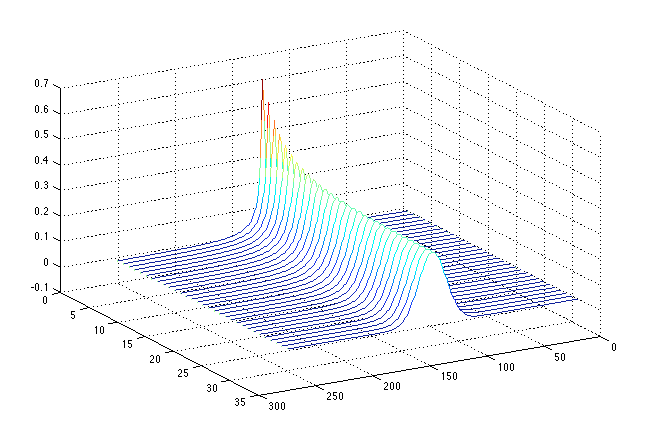
\includegraphics{/Users/willhahn/Research/alpha1.png}}     
\caption{Alpha-Stable Distributions as a function of Alpha}
\label{}
\end{figure}

\begin{figure}[h!]
\leavevmode      
\makebox{}\scalebox{.35}{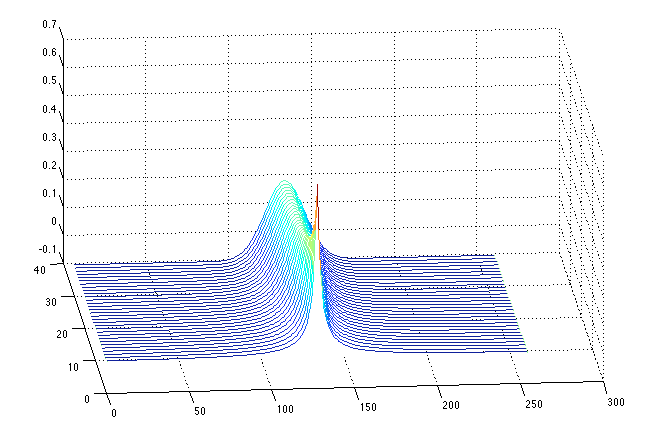
\includegraphics{/Users/willhahn/Research/alpha2.png}}     
\caption{Alpha-Stable Distributions as a function of Alpha}
\label{}
\end{figure}

\begin{figure}[h!]
\leavevmode     
\makebox{}\scalebox{.35}{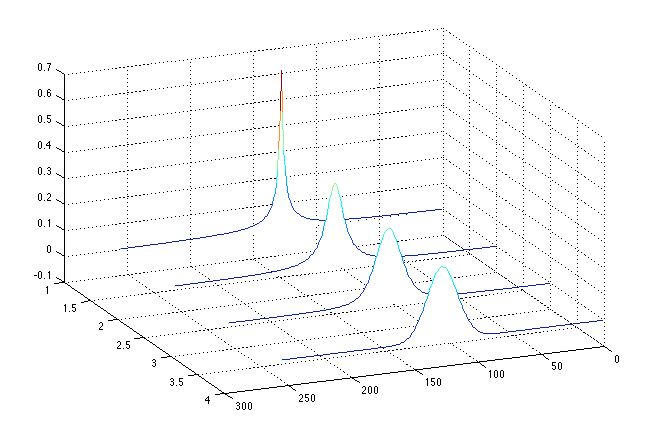
\includegraphics{/Users/willhahn/Research/alpha3.png}}     
\caption{Alpha-Stable Distributions as a function of Alpha}
\label{}
\end{figure}








\clearpage

\appendices
\section{Notes}





information gathering 

compressive sensing

scanpath

search strategy

forest vs meadow 

gaussian vs alpha stable

superclass of functions

no longer limited to special cases

analytical tools limit 

abstract search mechanisms

injection of noise into search algorithms

what type of noise is optimal

classically assumed that noise was a bug

maybe a feature 

mathematical search

search as random walk

markov chain 

optimization 

meta heuristic algorithms

nature uses noise and uncertainty to compute 

now we can measure 

without arbitrary thresholds 
 
characterize numerically 

applications 

characterizing human visual search behaviors

compression of images and video 

characterizing human and animal foraging and movement behaviors 

optimization and search algorithms

unmanned vehicles 

financial markets


knowing where humans are looking important for human computer interaction shared attention 





HVS

human visual system





MLE

fft

gpu




 saccadic mechanism

motor system implementation of an active random sampling strategy that the HVS has evolved in order to efficiently and effectively infer properties of the surrounding world. 



real time saliency fft on gpu demo

logo





  
Further these can be thought of Markov chains

CS has fewer parameter than PSO or Genetic Algorithms (GA)

network 

multi graph 

soft computing 

neural network np-complete 

corn field vector 

boids model 

collective intelligence

Boosting 

which goose known how to get to canada?

can a set of weak learners form a strong learner

wisdom of the crowds

natural parallelism 

scales to large number of processors each computing the fitness of a single particle location and communicating update to the global best to a common server asynchronously 

grand canyon 

fat tail distribution of noise 

most proposed changes will be small

similar to previous design 
 
at times large scale changes in parameters to shake up system dynamics and move out of local minima 

cooling schedule 

typically momentum term is lowered monotonically according to a described cooling schedule 

analog to the cooling of  solids crystals glasses metals 

glass blowing 

metal working 

ceramics

explore potential energy landscape 

temperature provides random noise that effectively proposes novel permutations of the system 

cooling forces a choice 

cooling slowly improves chance ending up in global minima 

advantage over metropolis hasting 

very long cooling times

random markov selection of new candidate 

advantage to use existing knowledge of energy landscape to constrain search 

orbit of dynamical system 

learning rule is a dynamical system

attractors 

fixed point at global minima 

basin of attraction 

stochastic gradient decent 

flocking behavior 

swarm algorithms 

social algorithm 

genetic algorithm 

geospatial metaphor 

flock towards optimal solution in n-dimensional space

perceptron

neural network 

non-linear threshold

weighted sum of inputs 

neuron fires if weighted sum excedes bias 

output set to one

activation function 

required to be differential for back propagation 

graph theory 

set of vertex or node 

set of edges 

directed weighted acyclic graph 

space of all possible graphs

fixed topology determines space of network weights

evaluation of proposed weight set is implemented though matrix multiplications and a nonlinear threshold operation 

elegant implementation in vector language such as Matlab

single line of code 

wrapper scripts to calculate error 

difference of network output with desired output 

supervised learning 

training set

testing set

validation 

mapping of input and output pairs 

network convergence

avoid over fitting 

multimodal optimization 

multiple feasible solutions 

find both corn fields 

matrix operations can be implemented on GPU for fast operation 

distribute swarm over many GPU/workstations and have separate central dedicated unit to rank fitness scores and distribute global best updates 

two stage search 

back propagation can be used at each particle location before fitness evaluation or back propagation can be preformed only on the global best to save resources.

even relatively large parameter space

transmission costs over a network for strings of n-bits

transmit global best over ethernet 

generate alpha-stable distribution 

no closed form solution exists 

numerical methods 

fast Fourier transform 

four parameter model 

different than method of moments  

gaussian distribution 

levy 

cauchy

special case of alpha-stable 

more general distributions allow heavy tails 

infinite variance  

meta optimization 

find alpha value that optimizes utility 

single gene genome 

particle swarm on one dimensional landscape 

swarm parameters can also determine network topology 

number of hidden units 

variety of feature units 

final weight indicate which features of the input provide the most information 

random walk 

levy flights 

levy distribution 

optimization as markov chain 

intensification 

diversification 

multiobjective

each node in the network 

related to many similar techniques 

genetic algorithms 

differential evolution

ant colony  

stigmergy 

krill herd 

firefly algorithm 

extreme learning machine 

only train output layer 

Optimization as Markov Chain

backpropagation swarm

The neural network

Particle swarm optimization

evaluations of fitness function are costly in time and space 

resources 

search 

cooperative search

explore energy landscape 

share information 

neighborhood

limited perceptual range

applications in real world search 

search and rescue 

multi-swarm 

random restart

APSO does not use velocity

swarm intelligence 

animal herds

bird flocking 

ant colonies 

bacterial growth biofilm 

fish schooling 

local minima

social interaction to problem solving

1995 by James Kennedy (social-psychologist) and Russell Eberhart (electrical engineer)

It uses a number of agents (particles) that constitute a swarm moving around in the search space looking for the best solution

Each particle is treated as a point in a N-dimensional space 

according to its own experience as well as the experience of other particles

personal best 

global best 

position
 
velocity

current searching point 

new searching point

current velocity 

new velocity

distance between current position and personal best 

distance between current position and global best 

selection mechanism 

crossover operation 

Stochastic Inputs



%%%%%%%%%%%%%%%%%%%%%%%%%%%%%%%%%%%%%%%%%%%%%%%%%%%%%%%%%

\clearpage

\bibliographystyle{IEEEtran}
\bibliography{IEEEabrv,Hahn_PSO_Paper_Bib}

\begin{IEEEbiographynophoto}{William Hahn}    
Received his undergraduate degree in Mathematics / Physics from Guilford College in North Carolina in 2008, with a research focus in flocking and swarm behavior before joining the Center for Complex Systems and Brain Sciences at Florida Atlantic University in 2011.
\end{IEEEbiographynophoto}
\begin{figure}[h!]
\leavevmode      
\makebox{}\scalebox{1}{\includegraphics{photo.png}}       
\end{figure}



\end{document}


